\section{Auswertung}

\subsection{Mittlere freie Weglänge}

In Tabelle \ref{tab:weg} befinden sich die mittleren freien Weglängen nach Gleichung \eqref{eqn:weg} $\bar{\omega}$ bei unterschiedlichen Temperaturen
und das Verhältnis $\frac{a}{\bar{\omega}}$, wobei der Abstand zwischen Kathode und Beschleunigungerelektrode als $a = \SI{1}{\cm}$
angenommen wird.
\input{Text/Tabellen/weg.tex}

\subsection{Skalierungsfaktoren}

Die aufgenommenen Messwerte aus Aufgabenteil a) befinden sich in Tabelle \ref{tab:skala} und die aufgenommenen Messwerte aus Aufgabenteil
b) und c) befinden sich in Tabelle \ref{tab:skalbc}.
\input{Text/Tabellen/skal.tex}
\input{Text/Tabellen/skal2.tex}

Aus diesen Messwerten ergeben sich folgende Skalierungsfaktoren:
\begin{align*}
  f_{a1} &= \SI{0,397(5)}{\V \per \cm} \\
  f_{a2} &= \SI{0,396(7)}{\V \per \cm} \\
  f_{b} &= \SI{2,902(146)}{\V \per \cm} \\
  f_{c} &= \SI{2,940(112)}{\V \per \cm} \\
\end{align*}

\subsection{Differentielle Energieverteilung und Kontaktpotential}
Der mithilfe des X-Y-Schreibers aufgenommene Graph bei $T = \SI{304,05}{\K}$ befindet sich in Abbildung \ref{fig:a1}.
\begin{figure}[H]
  \centering
  \includegraphics[width=.7\textwidth, angle=-90]{Text/Bilder/img001.jpg}
  \caption{Der mithilfe des X-Y-Schreibers aufgenommene Graph zur ersten Messung aus Aufgabenteil a) bei $T = \SI{304,05}{\K}$}
  \label{fig:a1}
\end{figure}

Die aus Abbildung \ref{fig:a1} abgelesenen Werte befinden sich in Tabelle \ref{tab:a1}.
\input{Text/Tabellen/a1.tex}

Aus diesen Werten ergibt sich Abbildung \ref{fig:a12}.
\begin{figure}[H]
  \centering
  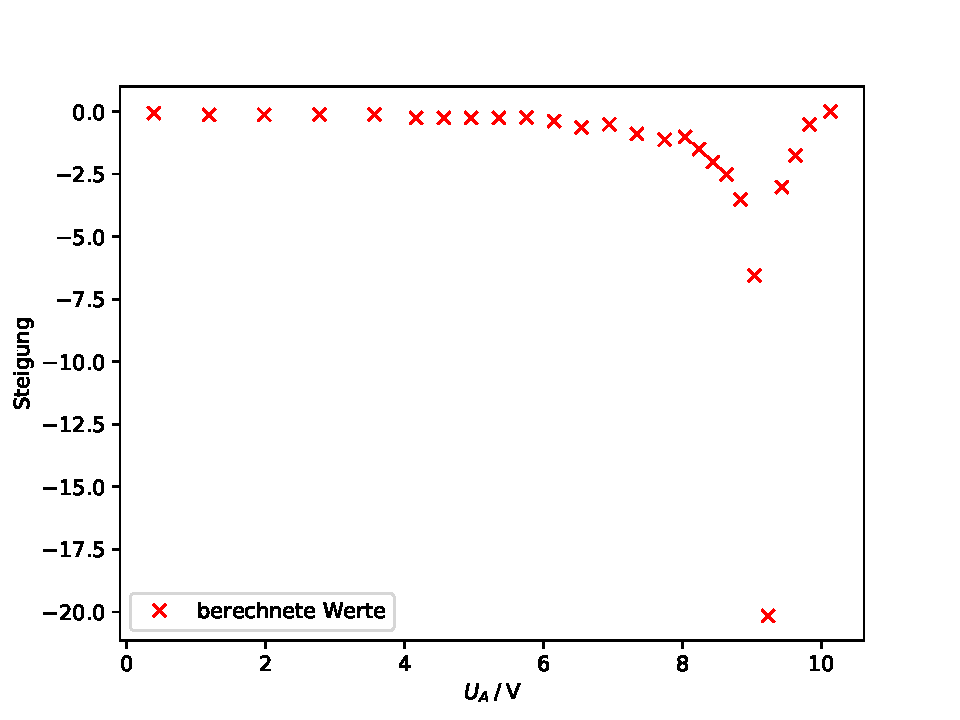
\includegraphics[width=.9\textwidth]{Plots/a1.pdf}
  \caption{Energieverteilung der Elektronen bei $T = \SI{304,05}{\K}$ und $U_B = \SI{11}{\V}$}
  \label{fig:a12}
\end{figure}

Der Peak liegt in Abbildung \ref{fig:a12} bei ca. $\SI{9,23}{\V}$. Somit beträgt das Kontaktpotential
\begin{equation*}
  K = \SI{11}{\V} - \SI{9,23}{\V} = \SI{1,77}{\V}.
\end{equation*}

Der aufgenommene Graph bei $T = \SI{423,15}{\K}$ befindet sich in Abbildung \ref{fig:a2}.
\begin{figure}[H]
  \centering
  \includegraphics[width=.7\textwidth, angle=-90]{Text/Bilder/img002.jpg}
  \caption{Der mithilfe des X-Y-Schreibers aufgenommene Graph zur zweiten Messung aus Aufgabenteil a) bei $T = \SI{423,15}{\K}$}
  \label{fig:a2}
\end{figure}

Aufgrund der höheren Temperatur steigt der Quecksilber-Dampfdruck. Infolgedessen nimmt die mittlere freie Weglänge der Atome ab und es
kommt zusätzlich zu elastischen Stößen zwischen den Elektronen und Hg-Atomen, wodurch die Elektronen abgelenkt werden und ihre Geschwindigkeit
(und daurch auch Energie) in Richtung der Auffängerelektrode sinkt. Desweiteren liegt die Energie der Elektronen bei einer
Beschleunigungsspannung von $U_\text{B} = \SI{11}{\V}$ über der Ionisierungsenergie von von Quecksilber. Aufgrunddessen kommt es zu unelastischen
Stößen bei denen die Elektronen einen großen Teil ihrer Energie verlieren.
\newpage
Die aus Abbildung \ref{fig:a2} abgelesenen Werte befinden sich in Tabelle \ref{tab:a2}.
\input{Text/Tabellen/a2.tex}

Aus diesen Werten ergibt sich Abbildung \ref{fig:a22}.
\begin{figure}[H]
  \centering
  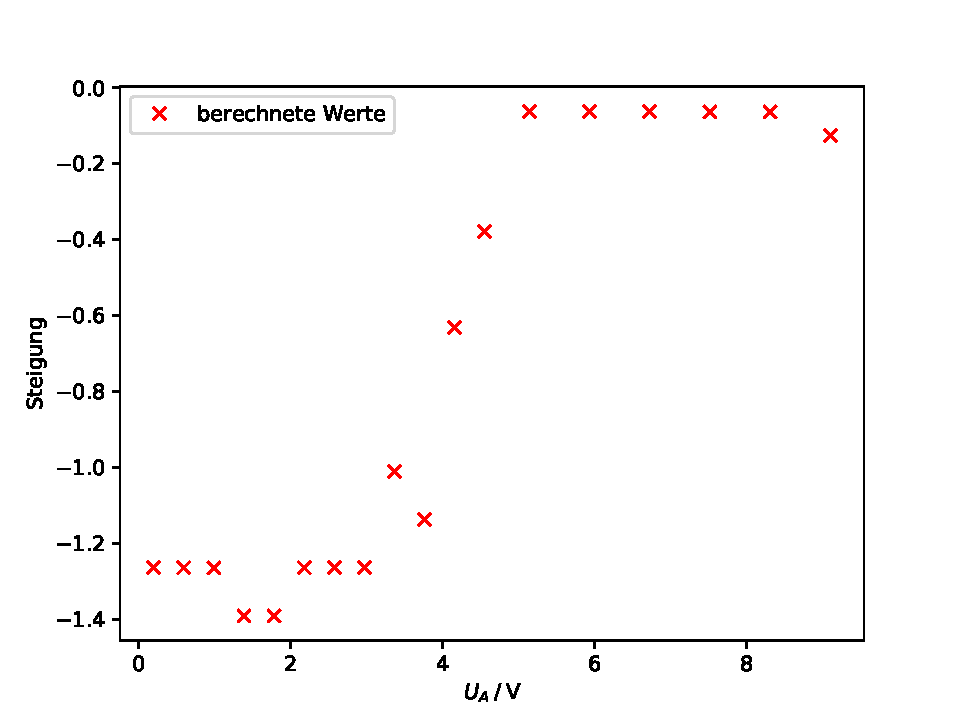
\includegraphics[width=.9\textwidth]{Plots/a2.pdf}
  \caption{Energieverteilung der Elektronen bei $T = \SI{423,15}{\K}$ und $U_B = \SI{11}{\V}$}
  \label{fig:a22}
\end{figure}

\subsection{Franck-Hertz-Kurve}
Die mithilde des X-Y-Schreibers aufgenommene Franck-Hertz-Kurve befindet sich in Abbildung \ref{fig:b}
\begin{figure}[H]
  \centering
  \includegraphics[width=.7\textwidth, angle=-90]{Text/Bilder/img003.jpg}
  \caption{Franck-Hertz-Kurve bei $T = \SI{442,15}{\K}$ und $U_A = \SI{1}{\V}$}
  \label{fig:b}
\end{figure}

In Tabelle \ref{tab:b} befinden sich die gemessenen Abstände zwischen den Peaks.
\input{Text/Tabellen/b.tex}

Diese werden mit dem Skalierungsfaktor $f_b$ multipliziert und mithilfe von \eqref{eqn:mit} und \eqref{eqn:sta} gemittelt.
\begin{align}
  \bar{x} &= \frac{1}{N} \sum_{i=1}^{N} x_i
  \label{eqn:mit} \\
  \Delta \bar{x} &= \sqrt{\frac{1}{N (N - 1)} \sum_{i=1}^{N} (x_i - \bar{x})^2}.
  \label{eqn:sta}
\end{align}

Für die erste Anregungsenergie ergibt sich dann $E_1 = \SI{4,85(9)}{\eV}$.
Der Literaturwert \cite{sample2} beträgt $E_{1, \text{theo}} = \SI{4,9}{\eV}$, somit ergibt sich eine Abweichung von $1,09 \%$.

Nach Gleichung \eqref{eqn:lam}
\begin{equation*}
  \lambda = \frac{h c}{E_1}
  \label{eqn:lam}
\end{equation*}
ergibt sich als abgestrahlte Wellenlänge $\lambda = \SI{255,81(460)}{\nm}$.

Der Fehler ergibt sich aus der Gauß'schen Fehlerfortpflanzung \eqref{eqn:gaus}
\begin{equation}
   \delta = \sqrt{ \sum_{i=1}^{n}(\frac{\partial y}{\partial x_i} \Delta x_i)^2}.
   \label{eqn:gaus}
 \end{equation}

\subsection{Ionisierungsenergie \label{sec:c}}
Der aufgenommene Graph befindet sich in Abbildung \ref{fig:c}
\begin{figure}[H]
  \centering
  \includegraphics[width=.7\textwidth, angle=-90]{Text/Bilder/img004.jpg}
  \caption{Der mithilfe des X-Y-Schreibers aufgenommene Graph zu Aufgabenteil c) bei $T = \SI{378,15}{\K}$}
  \label{fig:c}
\end{figure}

In Tabelle \ref{tab:c} befinden sich die aus Abbildung \ref{fig:c} abgelesenen Messwerte.
\input{Text/Tabellen/c.tex}

Aus diesen Messwerten ergibt sich Abbildung \ref{fig:c2}
\begin{figure}[H]
  \centering
  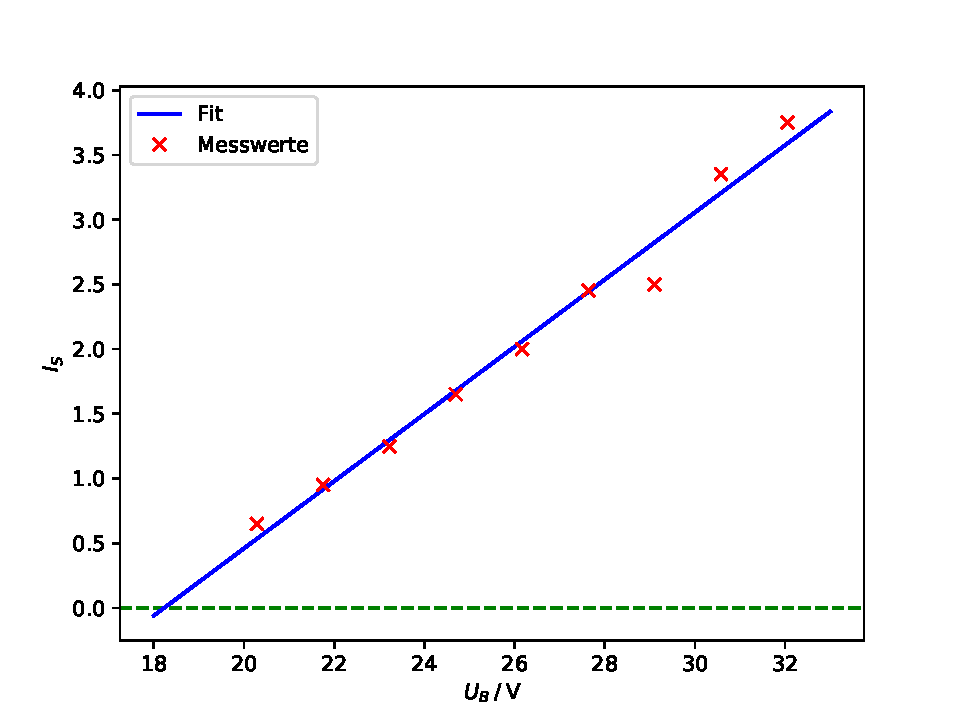
\includegraphics[width=.9\textwidth]{Plots/c.pdf}
  \caption{Graph zur Bestimmung der Ionisierungsenergie von Quecksilber bei $T = \SI{378,15}{\K}$ und $U_A = \SI{-30}{\V}$}
  \label{fig:c2}
\end{figure}

Dafür wurden die Messwerte auf $I_S = 0$ extrapoliert.
Mithilfe einer linearen Regression $f(x) = a \cdot x + b$ wird der Schnittpunkt mit der x-Achse berechnet.
Aus Gleichung \eqref{eqn:uion}
\begin{equation}
  U_\text{ion} + K = -\frac{a}{b}
  \label{eqn:uion}
\end{equation}

und der Gauß'schen Fehlerfortpflanzung \eqref{eqn:gaus} ergibt sich die Ionisierungsenergie
\begin{equation*}
  E_\text{ion} = \SI{16,46(171)}{\eV}.
\end{equation*}

Die Abweichung vom Literaturwert $E_{\text{ion}, \text{theo}} = \SI{10,437}{\eV}$ \cite{sample3} beträgt $58,00 \%$.
